\chapter{Introduction} \label{Chap1}
\section{Background}
In the intricate web of financial markets, market makers play a pivotal role. They are the cornerstone entities that ensure liquidity by continuously quoting bid and ask prices for various financial instruments. Market makers thrive on the principle of buying low and selling high, engaging in rapid and strategic trading activities to capitalize on price differentials within the market. Their prowess lies not only in the instruments they trade but also in the sophisticated strategies they employ to optimize their profit and loss (PnL) statements.

One of the key mechanisms through which market makers conduct trades is the request for quote (RFQ) system. RFQ serves as a fundamental protocol in over-the-counter (OTC) markets, allowing market participants to request quotes for specific quantities of financial instruments. Market makers respond with their bid and ask prices, creating a negotiation dynamic that culminates in a trade execution. The manner in which market makers navigate RFQs is a finely tuned art, involving rapid price assessments, risk management strategies, and acute market analysis. Their ability to swiftly quote competitive prices and execute trades while maintaining a profitable spread forms the cornerstone of their revenue generation model.

RFQ, in essence, acts as the lifeblood of OTC markets. Its importance reverberates across various financial sectors, including bonds, derivatives, and foreign exchange. Market makers leverage RFQs to optimize their PnL by not only offering competitive prices to secure trades but also by strategically managing their inventory and positions. The competitive edge in the financial landscape is not just about securing trades; it's about securing profitable trades. Market makers meticulously analyze market trends, pricing data, and trade history to predict market movements and quote RFQs that maximize their revenue potential.

\begin{figure}[ht]
    \centering
    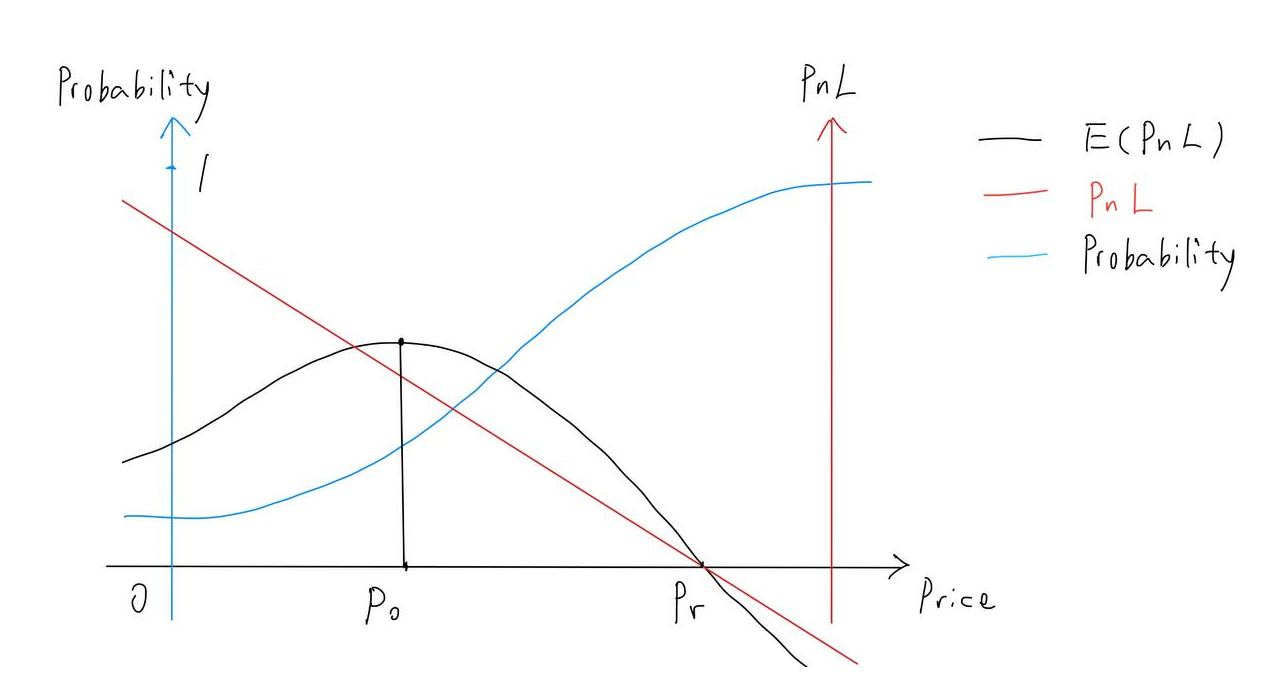
\includegraphics[width=0.8\textwidth]{figures/jpm/0. PnL of RFQs Curve.png}
    \caption{PnL of RFQs Curve}
    \label{fig:pnl_rfqs_curve}
\end{figure}

As illustrated in Figure \ref{fig:pnl_rfqs_curve}, the horizontal axis denotes the bid price, while the blue vertical axis on the left represents the transaction probability, and the red vertical axis on the right represents the market maker's Profit and Loss (PnL). The blue probability line indicates that transaction probability rises with increasing bid prices. Simultaneously, the corresponding red line reveals that the market maker's PnL diminishes as bid prices rise. The product of these two factors yields the expected PnL, portrayed by the black line. Initially, the expected PnL ascends and then descends, reaching its peak at $P_0$. Maximizing this expected PnL becomes a pivotal objective for the market maker. Determining the precise $P_0$ position emerges as a critical challenge.

It's worth noting that this study primarily focuses on the theoretical fit of the blue probability line and does not delve into trading simulation research or backtesting the red line's PnL. Nevertheless, understanding the interplay between bid prices, transaction probabilities, and resultant PnL is fundamental to optimizing market maker strategies.

Predicting the success of RFQs emerges as a pivotal challenge in this intricate ecosystem. The ability to forecast whether an RFQ will culminate in a trade execution carries immense implications for market makers' expected PnL. Accurate predictions empower market makers to strategically allocate resources, adjust pricing strategies, and optimize their trading activities. By anticipating the outcome of RFQ negotiations, market makers can proactively adapt their approaches, ensuring that their quotes not only secure trades but do so profitably. Thus, the ability to predict RFQ success becomes a keystone for market makers, shaping their trading decisions and revenue streams.

This research endeavors to delve into this critical aspect of financial analysis by harnessing the power of two distinct yet complementary survival analysis techniques: the Kaplan-Meier estimator and the Nelson-Aalen estimator. My goal is to not only estimate RFQ trade execution probabilities but also to understand the nuanced dynamics of this process over time.

The primary goal of this research is twofold: first, to employ two widely recognized survival analysis methods, namely the Kaplan-Meier estimator and the Nelson-Aalen estimator, to estimate the probability of success of RFQs in financial market; and second, to rigorously cross-validate these estimates against different time splits. The application of survival analysis techniques to RFQ estimation introduces a novel perspective into this domain, offering the potential to enhance the accuracy and robustness of predictions.

\section{Motivation and Rationale}
The motivation behind employing both the Kaplan-Meier and Nelson-Aalen estimators in this research is rooted in the need for comprehensive RFQ prediction.

In the context of estimating whether an RFQ will result in a trade being executed, we encounter a situation where the data comprises both uncensored and censored observations. Here, the survival analysis models, specifically the Kaplan-Meier and Nelson-Aalen estimators, offer a powerful framework for several reasons:

\subsection{Time-to-Event Analysis}
Survival analysis models are designed to handle time-to-event data, making them well-suited for estimating the probability of a future event, in this case, the execution of an RFQ.

\subsection{Censoring Handling}
Survival analysis can effectively account for censored data, which is essential in scenarios where RFQs may not have been executed within the observed time frame due to various reasons, such as unmatched prices, which account for the vast majority of the total data set. These censored data, representing RFQs that did not result in trades but were potentially viable, are crucial to understanding the overall trade execution probability.

The strength of survival analysis in dealing with censored data lies in its underlying statistical techniques. Unlike conventional statistical methods that consider only complete observations, survival analysis techniques incorporate censored data points, making them particularly relevant in situations where the event of interest is rare or takes a considerable amount of time to happen.

\subsection{Time-Price Relationship}
In the context of RFQ trade execution, the relationship between time and price is paramount. Survival analysis inherently considers time as a variable, and by matching it with the price component in the RFQ study, it allows for a nuanced examination of how price affects the likelihood of trade execution same as the estimating of how time affects the probability of event occurrence.

\subsection{Comparing Survival Curves}
By utilizing both the Kaplan-Meier estimator and the Nelson-Aalen estimator, which are variations of survival analysis, I can compare and contrast different aspects of RFQ trade execution. The Kaplan-Meier estimator is well-suited for estimating survival probabilities at specific time points, while the Nelson-Aalen estimator focuses on estimating the cumulative hazard function, which can provide insights into the overall trend of trade executions over time.

In summary, the Kaplan-Meier and Nelson-Aalen estimators are robust tools for estimating the probability that an RFQ will result in a trade being executed. Their ability to handle censored data, consider the time-price relationship, and provide a nuanced view of trade execution probabilities makes them valuable in my research on RFQ trade outcomes.

Furthermore, the backtesting phase of this study is pivotal in validating the practical effectiveness of RFQ estimations. Backtesting against various industries representing diverse market conditions and asset classes, and different time splits to depict validity among all folds, allows me to assess the adaptability and robustness of my estimators. The performance of these two estimators, informed by accurate RFQ trade results, is evaluated against the concordance index, hit rate and absolute maximum hit rate error, providing valuable insights into the practicality of my approach.

\section{Research Objectives}
In this study, I delve into the following pivotal research objectives:

Precision of Probability Estimations: Can the Kaplan-Meier estimator and Nelson-Aalen estimator accurately predict the probability of RFQ trade executions at varying time intervals, especially when dealing with censored price data that might witness more trade activities in the future? Additionally, what significant disparities exist in these estimations?

Comparative Analysis: How do these estimations measure up concerning accuracy and concordance? A comparative exploration is essential to understand the nuanced differences between the Kaplan-Meier and Nelson-Aalen estimators.

Insights Enrichment: To what degree do the insights derived from these estimators enrich my comprehension of RFQ trade execution probabilities within the dynamic landscape of financial markets? Understanding the depth of insights is crucial for applying these estimators effectively in practical financial scenarios.

By addressing these objectives, this study aims to contribute nuanced perspectives and enhanced understanding to the realm of survival analysis in the context of financial markets.

\section{Structure of the Paper}
This research paper is organized as follows: In Section 2, I conduct a comprehensive review of existing literature on RFQ estimation methods and backtesting in financial markets. Section 3 provide an in-depth exploration of the data utilized in my study and present detailed descriptive statistics. Section 4 outlines the methodology employed in this study, detailing the data sources, preprocessing steps, and the application of the Kaplan-Meier and Nelson-Aalen estimators. Section 5 presents the results of my analysis, while Section 6 delves into the discussion and interpretation of these findings and summarize my conclusions and propose avenues for further research.

As I embark on this journey into the realm of RFQ estimation and backtesting, I anticipate that my research will contribute valuable insights to the financial analysis community, ultimately aiding traders and decision-makers in navigating the complexities of modern financial markets.
